\chapter{Conclusion and Outlook}\label{ch:conOutlook}

A partially functioning MIMO experimental setup was achieved in this thesis. Firstly it is partial because of the dropped user data packets and secondly as its not a truely synchronised transmitter system. As explained in Section \ref{sssec:DLRXIQProc}, the hardware is not a true synchronous transceiver meaning that the 2 transmitting antennas are not time synchronised due to the phase differences in the RF paths. This is an extremely limiting factor in the ability to run custom MIMO experiments. Also given the limitations in the software and hardware delivered to MSV from NI, this was the best possible outcome with the hardware at hand. However with the modification listed below, better results could be achieved.

\section{FPGA File Port}\label{sec:FPGAChange}
Currently the FPGA Hardware design is where all the data is being received from the RF Front end and processed in real time. This FPGA hardware file is a pre compiled bit file delivered by NI to work with the older version of the LTE AFW Software. To adapt the design to suit the needs of the current research, the FPGA bit file has to be ported over to the latest version of Labview NXG to suit the design needs of the team.

\section{Transmitting User Defined Data}\label{sec:TransUserDefData}
Once the FPGA bit file has been modified, a user defined pattern can be transmitted through the shared data channel (PDSCH) instead of the CRS signals. The CRS signals were chosen as they were only a work around, and they enabled quick prototyping of the MIMO system without FPGA bitfile modification.

To be able to use the PDSCH channel, the implementation has to be changed to eliminate the data loss on the MIMO systems. Once the source of the packet drop has been identified, a pseudo random pattern with a fixed seed can also be generated and sent over the air. Finally there is also the possibility of sending custom bit streams over the air.

\section{Experiments with structured Channel}\label{sec:StrucChannel}
Structured channels could first be built using reflectors, instead of having a single Line of Sight (LOS) channel. The structure of the channel can be verified (using a Singular Value Decomposition of the channel matrix) if and only if all the channel coefficients are available. Once this channel has been created, experiments can be run for with this channel.

\section{Wideband Antennas}\label{sec:WdBdAntennas}

Figure \ref{fig:HandSAnt} shows an omni directional Antenna from Huber and Suhner (SWA-
2459/360/4/45/V), which is capable of transmitting and receiving in the frequency range of 2400MHz to 5875MHz. The antenna also has an antenna gain of 4dBi which is important to compensate for some losses. These experiments can be useful potentially in the higher frequency bands. Although the USRP2940 can only transmit upto 2.2\si{\giga\hertz}, it can be replaced with other USRPs as defined in Table \ref{tb:USRPPartsList} that can transmit up to 6\si{\giga\hertz}

\begin{figure}[!htb]
    \centering
    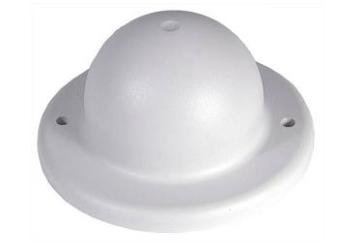
\includegraphics[width=10cm]{images/HuberAntenna.png}
    \caption{Huber and Suhner SWA-2459/360/4/45/V widebadn Antenna}
    \label{fig:HandSAnt}
\end{figure}

%TODO add photos of the missing dependencies
% Add Huber und Suhner Antenna photo
